\chapter{Data Preprocessing}
\label{cha:Preprocessing}


According to \cite[p.~99]{raschka} the quality of data as well as the amount of useful information which is contained in data are crucial factors for the performance of a machine learning algorithm. Therefore, data has to be examined, preprocessed and understood before it can be used. The data used in this project is provided in a SQLite databse and has the following entity relationship modell:

\begin{figure}[H]
\label{fig:ERM}
\begin{center}
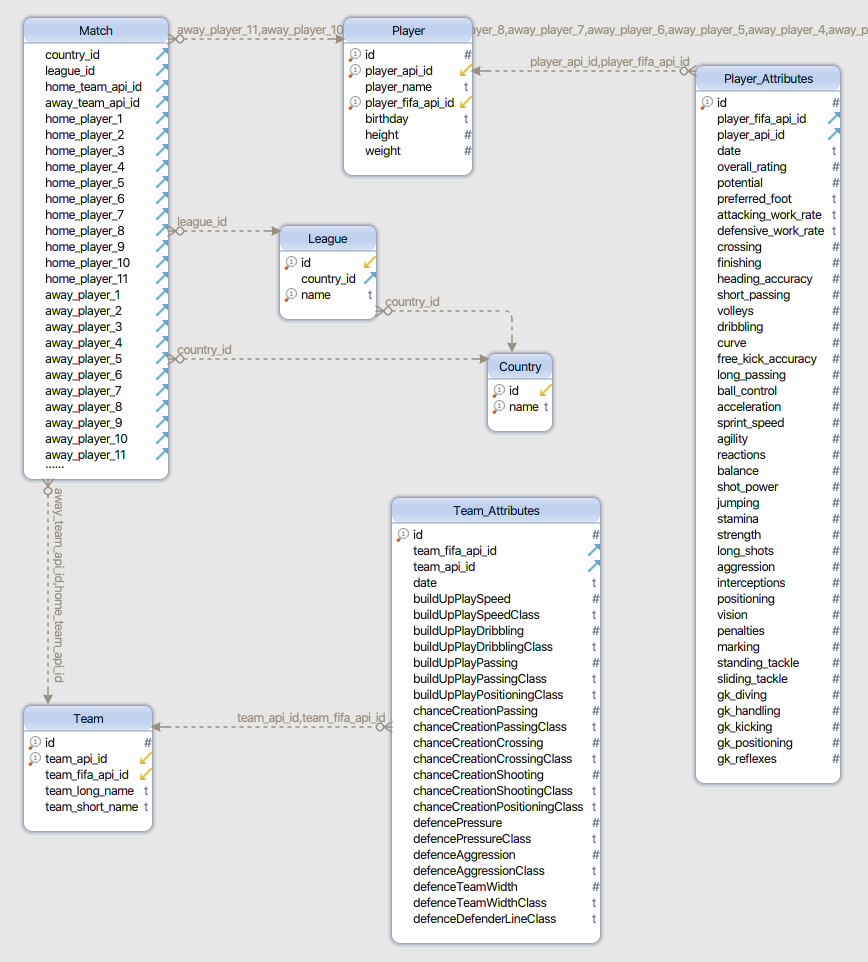
\includegraphics[scale=.5]{erm} % png ist Default für Dateiendung
\end{center}
\caption{Entity Relationship Modell European Soccer Database
%  \parencite[eigene Darstellung mit Übersezung in Anlehnung an][]{Hevner2007}
}
\end{figure}


